\section{Introduction}

Pour mon stage de fin de licence, j'avais un stage de 7 semaine a effectué en entreprise ou en laboratoire en fonction de si l'on voulais s'inserer dans le monde proffestionel ou academic. Pour ma part, car je souhait m'orienter vers une parocurs profetionel, j'ai choisi de faire mon stage en entreprise a Orano.
\subsection{Orano}
Orano est un grand group français spécialisée dans le nucléaire. Elle possede 17 500 collaborateur dans 17 pays et avait un revenu de 4.8 M en 2023\cite{report:rapport_activiter}. Elle est née en 2018 a la suite d'une restructurisation d'areva. Elle est présente dans plusieurs domaines du nucléaire, de l'extraction de l'uranium à la gestion des déchets nucléaires en passant par la production de combustible nucléaire. Ses différentes activiter sont répartie dans plusieurs filiales~:
\begin{description}
    \item [Orano Support] qui regroupe les activités de support du groupe
    \item [Orano Mining] qui regroupe les activités d'extraction d'uranium
    \item [Orano Medical] qui regroupe les activités de production de radioéléments pour la médecine nucléaire
    \item [Orano Batteries] qui regroupe les activités de recyclage de batterie
    \item [Orano Dismantling] qui regroupe les activités de démantèlement de centrale nucléaire
    \item [Orano Chimie-Enrichissement] qui regroupe les activités de chimie et d'enrichissement de l'uranium
\end{description}
\begin{figure}
    \centering
    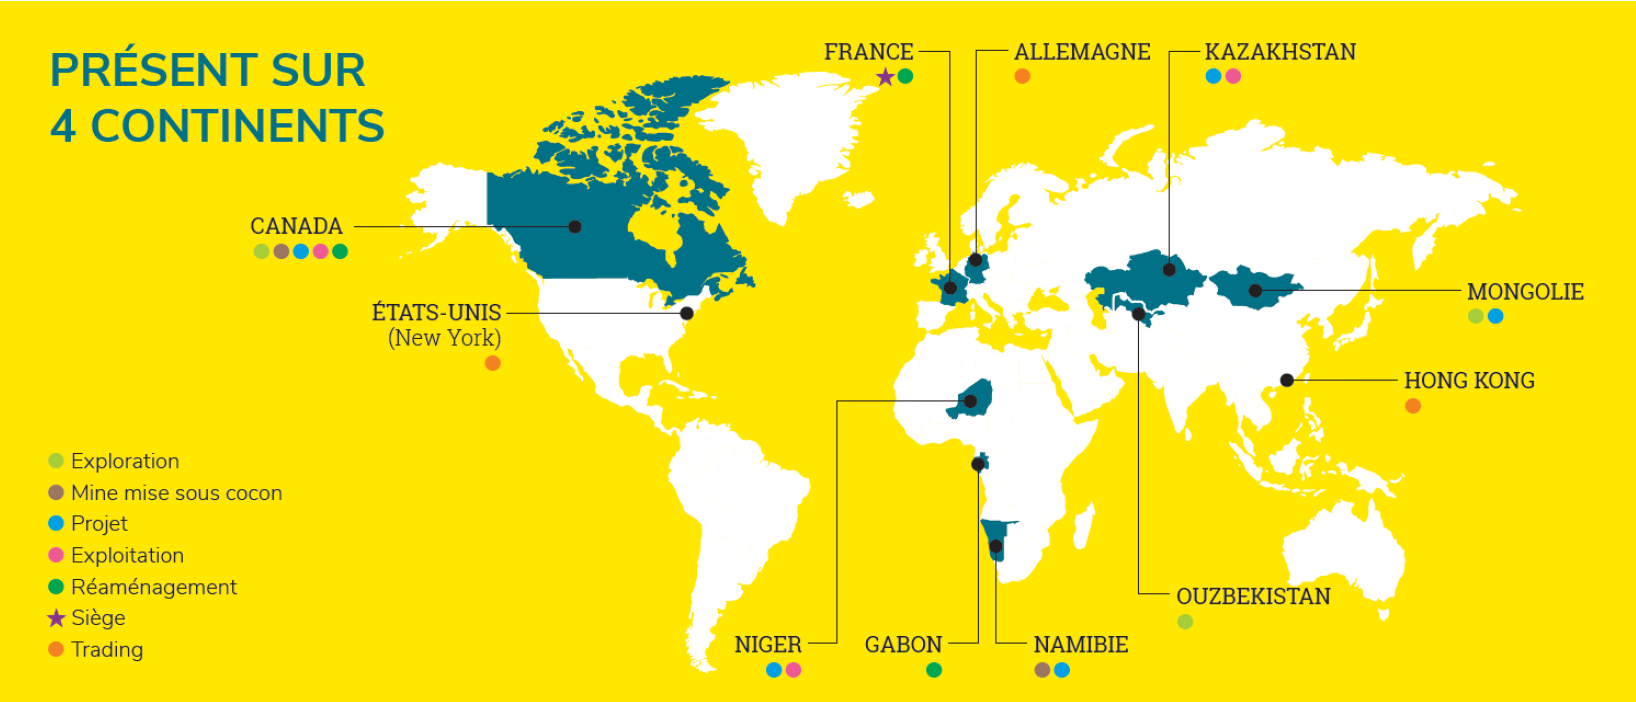
\includegraphics[width=0.5\textwidth]{img/Carte-ornao-international.png}
    \caption{Carte des activités d’Orano Mining dans le monde, Source~:~Dossier d’information Orano 2020}
    \label{fig_carte_orano}
\end{figure}









ces filliale sont présente a l'international avec des mines d'uranium au Kazakhstan, au Canada et au Niger, de l'exploration ou des projet en Namibie, en Ouzebekistan et en Mongolie. La majoriter des site a l'etranger d'Orano sont des site d'Orano Mining due a la nature de ses activiter. C'est dans cette dernière que j'ai effectué mon stage.
\subsection{Orano Mining}

Orano mining est en charge de tous ce qui est relatif a l'extraction de l'uranium. Nous pouvont repartir ses activiter en 3 grand domaines~:
\subsubsection{L'exploration}
L'exploration est la première étape de l'extraction de l'uranium. Elle consiste a trouver des gisement d'uranium. Pour cela, Orano Mining utilise des méthode géophysique et géochimique pour trouver des gisement d'uranium. Une fois un gisement trouvé, il faut l'exploiter.

\subsubsection{L'exploitation}
L'exploitation est la deuxième étape de l'extraction de l'uranium. Elle consiste a extraire l'uranium du sol. Pour cela, Orano Mining utilise diverse methode d'extraction en fonction de la nature du gisement. On peut citer~:
\begin{description}
    \item [L'extraction in situ] qui consiste a injecter de l'acide dans le sol entre deux couche etanche pour dissoudre l'uranium et le remonter a la surface (voir \cref{ssec_insitu}). C'est le cas des mines de Muyunkum et Tortkuduk au Kazakhstan.
    \item [L'extraction par jetboring] qui consiste a creuser un trou dans le sol et a injecter de l'eau sous pression pour remonter l'uranium a la surface (voir \cref{ssec_jetbore}). C'est le cas de la mine Cigar Lake au Canada.
    \item [L'extraction par raisebore et boxbore] qui consiste a forer par en dessous de gisment pour le laiser retomber dans la galerie pricipal(voir \cref{ssec_raisebore,ssec_boxbore}). C'est le cas de la mine McAthure River au Canada.
    \item [L'extraction a ciel ouvert] qui consiste a creuser une fosse pour extraire l'uranium. C'est le cas de la mine de Somaïr au Niger et de Mclean Lake au Canada (production suspendu entre 2008 et 2025 a cause de la chute du cours de l'uranium).
\end{description}

\subsubsection{Le traitement}
Le traitement est la dernière étape de l'extraction de l'uranium. Elle consiste a traiter le minerai pour en extraire l'uranium. Pour cela, Orano Mining utilise des méthode de traitement chimique pour extraire l'uranium du minerai. Generalement, cette etap est faite avec une  lixiviation de l'uranium por une solution concentre acidique, alkaline ou de peroxide pour former ce que l'on appelera du yellow cake due a sa couleur et texture (voir \cref{fig_yellow-cake}). Le yellow cake est composer entre 70\% et 90\% d'oxide d'urnaium notament d'$U_3O_8$ \cite{article:composition-yellow-cake}. Une fois l'uranium extrait, il est envoyé a Orano Chimie-Enrichissement ou a d'autre partenaire pour être enrichi. En effet l'uranium naturel est composé a 0,7\% d'uranium 235 et a 99,3\% d'uranium 238\cite{}. Pour être utilisé dans un réacteur, il faut que l'uranium 235 soit enrichi entre 3\% a 5\% \cite{article:uranium-concentration}

\begin{figure}
    \centering
    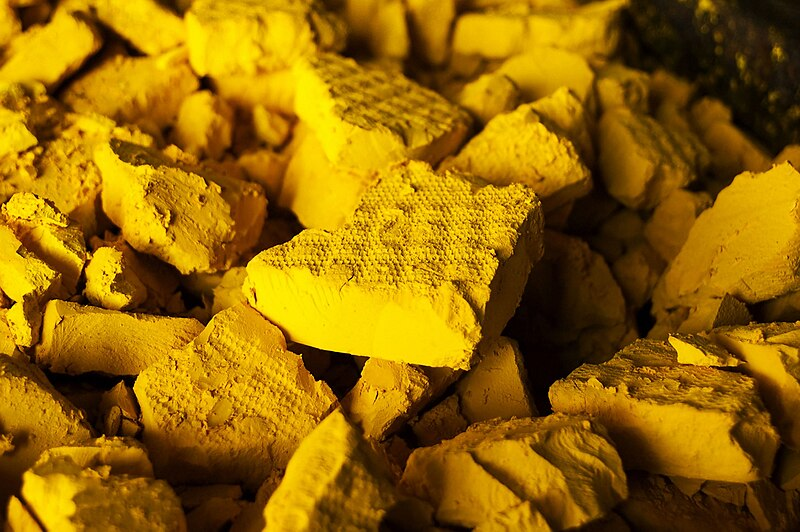
\includegraphics[width=0.5\textwidth]{img/Yellow_Cake_Uranium_(14492248719).jpg}
    \caption{Apparence de yellow cake. Avec des methode modern certain taritemetn peuve lui donnée une apparence marrow voir noir. Source~:~\href{https://commons.wikimedia.org/wiki/File:Yellow_Cake_Uranium_(14492248719).jpg}{Nuclear Regulatory Commission from US}, Public domain, via Wikimedia Commons}
    \label{fig_yellow-cake}
\end{figure}

\subsubsection{L'apres mine}
L'apres mine designe l'ensemble d'action de remediation de monitoring qui sont entre pris par Orano apres qu'une mine ferme. En effet, une fois une mine fermée, il faut la remettre en état pour éviter les risque de pollution. Pour cela, Orano Mining met en place des systeme de monitoring pour surveiller l'évolution de la mine et des action de remediation pour remettre la mine en état. En france, Orano a la charge de 235 sur 247 des site minier d'uranium present sur le territoire dont des site que les ancetre d'orano n'ont pas exploiter \cite{site:orano_apres_mine}. L'apres mine n'intervient pas que en france mais aussi a l'etranger. Par exemple, au Canada, Orano a finit la remediation de la mine de Cluff Lake (1979-2002) en 2013 et le site a etait ouvert au publique \cite{site:Cluff_lake_remediation}.

\subsection{Direction de la transformation digital}
Au sein de la mine est un petit service qui est en charge de la transformation digital de la mine. Ce service est en charge de mettre en place divers outils digital pour améliorer les procedure de la mine. Pour cela, il travaille en collaboration avec les différent service de la mine pour comprendre leur besoin et mettre en place des outils qui répondent a leur besoin. C'est dans ce service que j'ai effectué mon stage.